% vim:spell spelllang=sk
\section{Decimácia v čase radix2}

Pretým, než si ukážeme tento algoritmus, objavíme najskôr
krásu motýlích krídel\footnote{Z anglického názvu ``Butterfly''}.
To, čo robí štandardný DFT algoritmus pomalým, je jeho ignorancia.
Ignoruje totiž 2 veľmi dôležité fakty o komplexných koreňoch $\omega$,
ktorými sú
\begin{itemize}
 \item Symetria: $\omega_{n,k+n/2} = -\omega_{n,k}$, ak je $n$ párne
 \item Periodicita: $\omega_{n,k+n} = \omega_{n,k}$
\end{itemize}
Ich všímavým pozorovaním môžeme dospieť napríklad k nasledujúcemu
faktu:
\begin{equation}
\begin{split}
X_k & = \sum_{l=0}^{n-1} x_l \omega_{n,kl}, \qquad k=0,1,\dots,n-1 \\
    & = \sum_{l \rm{\:je\:párne}} x_l \omega_{n,kl}
      + \sum_{l \rm{\:je\:nepárne}} x_l \omega_{n,kl} \\
    & = \sum_{l=0}^{\lceil n/2 \rceil-1} x_{2l} \omega_{n,2kl} 
      + \sum_{l=0}^{\lfloor n/2 \rfloor-1} x_{2l+1} \omega_{n,k(2l+1)}
\end{split}
\end{equation}
V ďalšom texte budeme automaticky uvažovať prípad, že $n$ je párne.
Využijeme rovnosť $\omega_{n,k}^2 = \omega_{n/2,k}$ a výsledok upravíme na
tvar
\begin{equation}
\begin{split}
X_k & = \sum_{l=0}^{n/2-1} x_{2l} \omega_{n/2}^{kl} 
      + \omega_{n,k} \sum_{n=0}^{n/2-1} x_{2l+1} \omega_{n/2,kl}
\end{split}
\end{equation}
Nech $y_n=x_{2n}, \quad z_n=x_{2n+1}$. Potom 
$X_k = Y_k + \omega_{n,k} Z_k, k\in0,1,\dots,n-1$,
kde $Y_k, Z_k$ sú $n/2$ bodové diskrétne Furierove transformácie
postupností $x$, resp. $y$ s periódou $n/2$, teda $Y_{n/2+k} = Y_k,
Z_{n/2+k} = Z_k$. 
Využitím periodicity a faktu $\omega_{n,n/2+k} = -\omega_{n,k}$
dostaneme
\begin{align}
 X_k &= Y_k + \omega_{n,k} Z_k \quad& , k\in0,1,\dots,n/2-1 \\
 X_{n/2+k} &= Y_k - \omega_{n,k} Z_k,\quad& k\in0,1,\dots,n/2-1 \\
\end{align}

Schématický výpočet $X_k, X_{n/2+k}$ z $Y_k, Z_k$ vidno na
diagrame \ref{fig:butterfly_dit}, z ktorého pochádza motýlí názov.
\begin{figure}[htp]
    \centering
        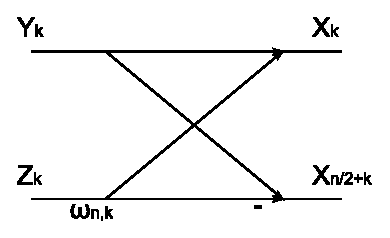
\includegraphics{obrazky/algoritmy/butterfly_dit}
        \caption{Butterfly diagram pre decimáciu v čase}
    \label{fig:butterfly_dit}
\end{figure}

K algoritmu už nie je dlhá cesta. Ak predpokladáme, že $n$ je mocnina
dvojky, vieme postupnosti $Y,Z$ vypočítať rekurzívne presne tým istým
algoritmom. Časová zložitosť algoritmu je $O(n\log n)$ ako sa môžeme
ľahko presvedčiť, nakoľko platí $T(n) = 2 T(n/2) + O(n)$.
Faktor o ktorom sme zatiaľ nehovorili je pamäť. Pri bežnom rekurzívnom
prístupe bude jej veľkosť taktiež $O(n \log n)$. Algoritmus sa ale
jednoducho dá zmeniť na "in-place" algoritmus, ktorý okrem vstupného
poľa bude potrebovať len konštantne veľa pamäti. Pozrime sa opäť na
výpočet algoritmu, tentokrát aj s rekurzívnymi volaniami pre $n=8$ ako
je znázornené na ilustrácii \ref{fig:dit}

\begin{figure}[htp]
    \centering
        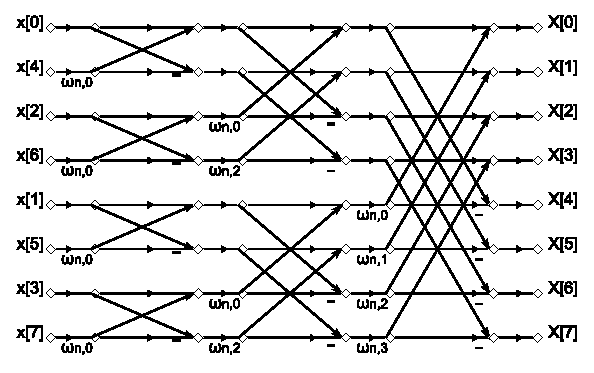
\includegraphics{obrazky/algoritmy/dit}
        \caption{Výpočet decimácie v čase pre $n=8$}
    \label{fig:dit}
\end{figure}

Môžeme vidieť, že hodnoty $x_k$ sa používajú len v poslednom kroku
rekurzie, ich výstup sa používa len v predposlednom kroku rekurzie
atď. Algoritmus teda vieme prepísať jednoducho bez rekurzie.
Prvým krokom pred priamym výpočtom je je takzvané "bit reversal"
preusporiadanie. Je jednoduché zhliadnuť, že ak $k$ má binárny zápis
$b_{m-1} b_{m-2} \dots b_1 b_0$ kde $m = \log_2 n$, potom musíme
$x_k$ presunúť na pozíciu $b_0 b_1 \dots b_{m-2} b_{m-1}$. Jednoduchý
dôkaz tohoto tvrdenia: 
Predpokladajme, že chceme vypočítať $X_k, X_{n/2+k}$. Ak si povieme,
že použijeme (vypočítané) hodnoty $Y_k, Z_k$ a chceme aby zmena bola
na mieste, môžeme povedať, že $Y_k$ bude na mieste $X_k$ a $Z_k$ bude
na mieste $X_{n/2+k}$. Dáta pre $Y$ sa teda nachádzajú v prvoj
polovici poľa, zatiaľ čo dáta pre $Z$ v druhej polovici.
Keď si spomenieme, potrebné dáta na vypočítanie $Y$ sú práve tie $x_i$ kde $i$ je párne,
a dáta pre $Z$ tie, kde $i$ je nepárne. Teda, pred posledným krokom
musia byť najskôr všetky párne a potom všetky nepárne údaje. Keď sa
teraz pozrieme na výpočet $Y$ a $Z$, môžeme vidieť, že dáta v rámci
každej z týchto polovíc vstupu musia mať najskôr 2. bit nulový, a až
potom nasledujú údaje s 2. bitom nenulovým. Opakovaním tohoto postupu
nakoniec dôjdeme k spomínanému tvrdeniu o bitovom reverze.

\begin{python}
import cmath
import math
from bitutils import BitUtils

class DIT:
    def transformInPlace(data):
        n = len(data)
        assert(BitUtils.isPowerOf2(n))

        BitUtils.bitReverseInPlace(data)

        skip = 2

        while skip <= n:
            for block in range(n/skip):
                for i in range(skip/2):
                    # do butterfly
                    y = data[block * skip + i]
                    z = data[block * skip + skip/2 + i]
                    k = i * (n/skip)
                    twiddle = cmath.exp( -2 * 1j * math.pi / n * k)
                    data[block * skip + i] = y + twiddle * z
                    data[block * skip + skip/2 +i] = y - twiddle * z
            skip *= 2


    transformInPlace = staticmethod(transformInPlace)
\end{python}    


\todo{cite:dit}
